
% ----------------------------------------------------------------------------
%                           Document of oral presentation
%                                   口試証明文件
% ----------------------------------------------------------------------------

% ----------------------------------------------------------------------------

\ifthenelse{\OralDocument = \OralDocumentTemplete}
{
  % 顯示範本
  \ifthenelse{\OralDocumentEngOnly = 0}
  {
    % Page start
    \newpage
    \phantomsection

    % 設定顯示在目錄
    \addcontentsline{toc}{chapter}{Document of oral presentation}

    % Chinese version
    %
% This file is part of ncku-thesis-template.
%
% ncku-thesis-template is distributed in the hope of usefuling to someone,
% you can redistribute it and/or modify
% it under the terms of the Attribution-NonCommercial-ShareAlike
% 4.0 International.
%
% You should have received a copy of the
% Attribution-NonCommercial-ShareAlike 4.0 International
% along with ncku-thesis-template.
%
% If not, see <http://creativecommons.org/licenses/by-nc-sa/4.0/legalcode.txt>.
%

% ----------------------------------------------------------------------------
%   Document of oral presentation (Chinese version)
%                   中文版口試証明文件
% ----------------------------------------------------------------------------

% Set the line spacing to single for the titles (to compress the lines)
\renewcommand{\baselinestretch}{1}   %行距 1 倍

% 由於中文版的watermark是用文字, 所以先把Logo版關掉
\ClearWatermark

% ------------------------------------------------

% Page start
% Add to "Table of Contents"
% 設定使用 無頁碼, 有浮水印
\newpage
\phantomsection
\addcontentsline{toc}{section}{Chinese version}
\thispagestyle{empty}

% 使用文字版watermark
\UseSchoolTextWatermark

% Aligned to the center of the page
\begin{center}

% ------------------------------------------------

% 顯示 校名, 論文種類
\makebox[\textwidth][c]{\Huge \GetSchoolChiName}\\
\vspace{0.5cm}
\makebox[\textwidth][c]{\Huge \GetChiDegree 論文}\\

% ------------------------------------------------

\vspace{0.8cm}

% ------------------------------------------------

% Chinese and English title 中英文題目
\begin{minipage}[c][3cm][c]{\textwidth}
  \begin{center}
%    \parbox{\paperwidth}{\center \Large \GetChiTitle}
%    \parbox{\paperwidth}{\center \Large \GetEngTitle}
    \makebox[\textwidth][c]{\parbox{\paperwidth }{\center \Large \GetChiTitle}}
    \makebox[\textwidth][c]{\parbox{\paperwidth }{\center \Large \GetEngTitle}}
  \end{center}
\end{minipage}

% ------------------------------------------------

\vspace{0.5cm}

% ------------------------------------------------

% 顯示 學生 的名字
\hspace{2.4em}
\makebox[4.8em][r]{\Large 研究生:}
\makebox[7.2em][l]{\Large \GetAuthorChiName} \\

% --------------------------
\vspace{0.5cm}
\makebox[\textwidth][c]{\Large 本論文業經審查及口試合格特此證明} \\
% --------------------------

% 博士學位考試委員會置委員五人至九人
% 碩士學位考試委員會置委員三人至五人
% 口試委員人數含指導教授

\vspace{1.0cm}
\begin{minipage}[c][8.0cm][t]{\textwidth}
  \makebox[\textwidth][l]{\Large 論文考試委員:} \\
  \DisplayCommitteeSignatureArea
\end{minipage}

% ------------------------------------------------

% Space
\vspace{0.5cm}

% ------------------------------------------------

\makebox[4.8em][r]{\Large 指導教授}
\makebox[1em][c]{\Large:}
\makebox[7.2em][l]{\namesigdate}\\

\vspace{0.8cm}

\makebox[4.8em][r]{\Large 系(所)主管}
\makebox[1em][c]{\Large:}
\makebox[7.2em][l]{\namesigdate}\\

% --------------------------

% Date 日期
\vspace{1.0cm}
\makebox[\textwidth][s]{\Large 中華民國 \GetOralChiYear 年 \GetOralChiMonth 月 \GetOralChiDay 日}

% ------------------------------------------------

% End of alignment
\end{center}

% End of page
\clearpage

% 重新使用學校浮水印 Watermark
\UseSchoolWatermark
% ------------------------------------------------


    %
% This file is part of ncku-thesis-templete.
%
% ncku-thesis-templete is distributed in the hope that it will be useful,
% you can redistribute it and/or modify
% it under the terms of the Attribution-NonCommercial-ShareAlike
% 4.0 International.
%
% You should have received a copy of the
% Attribution-NonCommercial-ShareAlike 4.0 International
% along with ncku-thesis-templete.
%
% If not, see <http://creativecommons.org/licenses/by-nc-sa/4.0/legalcode.txt>.
%

% ----------------------------------------------------------------------------
%   Document of oral presentation (Chinese version)
%                   中文版口試証明文件
% ----------------------------------------------------------------------------

% Set the line spacing to single for the titles (to compress the lines)
\renewcommand{\baselinestretch}{1}   %行距 1 倍

% 由於中文版的watermark是用文字, 所以先把Logo版關掉
\ClearWatermark

% ------------------------------------------------

% Page start
% Add to "Table of Contents"
% 設定使用 無頁碼, 有浮水印
\newpage
\phantomsection
\addcontentsline{toc}{section}{Chinese version 2}
\thispagestyle{empty}

% 使用文字版watermark
\UseSchoolTextWatermark

% Aligned to the center of the page
\begin{center}

% ------------------------------------------------

% 顯示 校名, 論文種類
\makebox[\textwidth][c]{\Huge \GetSchoolChiName}\\
\vspace{0.5cm}
\makebox[\textwidth][c]{\Huge \GetChiDegree 論文}\\

% ------------------------------------------------

\vspace{2.0cm}

% ------------------------------------------------

% Chinese and English title 中英文題目
\begin{minipage}[c][3cm][c]{\textwidth}
  \begin{center}
    \parbox{\textwidth}{\center \Large \GetChiTitle}
    \parbox{\textwidth}{\center \Large \GetEngTitle}
    {\Large (口試文件版本2 - 等待認可)}
  \end{center}
\end{minipage}

% ------------------------------------------------

\vspace{2.2cm}

% ------------------------------------------------

% 顯示 學生 的名字
\hspace{2.4em}
\makebox[4.8em][r]{\Large 研究生:}
\makebox[7.2em][l]{\Large \GetAuthorChiName} \\

% --------------------------
\vspace{1.0cm}
\makebox[\textwidth][c]{\Large 本論文業經審查及口試合格特此證明} \\
% --------------------------
\vspace{1.0cm}
\makebox[11.6cm][l]{\Large 論文考試委員:} \\
% --------------------------

\vspace{4.5cm}
\hspace{2.4em}
\makebox[4.8em][r]{\Large 指導教授:}
\makebox[7.2em][l]{}

\vspace{0.5cm}
\hspace{2.4em}
\makebox[4.8em][r]{\Large 系(所)主管:}
\makebox[7.2em][l]{}

% --------------------------

% Date 日期
\vspace{0.5cm}
\makebox[\textwidth][s]{\Large 中華民國 \GetOralChiYear 年 \GetOralChiMonth 月 \GetOralChiDay 日}

% ------------------------------------------------

% End of alignment
\end{center}

% End of page
\clearpage

% 重新使用學校浮水印 Watermark
\UseSchoolWatermark

% ------------------------------------------------


    
% ----------------------------------------------------------------------------
%   Document of oral presentation (Chinese version)
%                   中文版口試証明文件
% ----------------------------------------------------------------------------

% Set the line spacing to single for the titles (to compress the lines)
\renewcommand{\baselinestretch}{1}   %行距 1 倍

% ------------------------------------------------

% Page start
% Add to "Table of Contents"
% 設定使用 無頁碼, 有浮水印
\newpage
\phantomsection
\addcontentsline{toc}{section}{Chinese version 3}
\thispagestyle{empty}

% Aligned to the center of the page
\begin{center}

% ------------------------------------------------

% 顯示 校名, 論文種類
\makebox[\textwidth][c]{\Huge \GetSchoolChiName}\\
\vspace{0.5cm}
\makebox[\textwidth][c]{\Huge \GetChiDegree 論文}\\

% ------------------------------------------------

\vspace{2.0cm}

% ------------------------------------------------

% Chinese and English title 中英文題目
\begin{minipage}[c][3cm][t]{\textwidth}
  \begin{center}
    \Large \GetChiTitle \\
    \Large \GetEngTitle \\
    (口試文件版本3 - 等待認可)
  \end{center}
\end{minipage}

% ------------------------------------------------

\vspace{2.2cm}

% ------------------------------------------------

% 顯示 學生 的名字
\hspace{2.4em}
\makebox[4.8em][r]{\Large 研究生:}
\makebox[7.2em][l]{\Large \GetAuthorChiName} \\

% --------------------------
\vspace{1cm}
\makebox[\textwidth][c]{\Large 本論文業經審查及口試合格特此證明} \\
% --------------------------
\vspace{1cm}
\makebox[11.6cm][l]{\Large 論文考試委員:} \\
% --------------------------

\vspace{4.5cm}
\hspace{2.4em}
\makebox[4.8em][r]{\Large 指導教授:}
\makebox[7.2em][l]{}

\vspace{0.5cm}
\hspace{2.4em}
\makebox[4.8em][r]{\Large 系(所)主管:}
\makebox[7.2em][l]{}

% --------------------------

% Date 日期
\vspace{0.5cm}
\makebox[\textwidth][s]{\Large 中華民國 \GetOralChiYear 年 \GetOralChiMonth 月 \GetOralChiDay 日}

% ------------------------------------------------

% End of alignment
\end{center}

% End of page
\clearpage
% ------------------------------------------------


    
% ----------------------------------------------------------------------------
%   Document of oral presentation (Chinese version)
%                   中文版口試証明文件
% ----------------------------------------------------------------------------

% Set the line spacing to single for the titles (to compress the lines)
\renewcommand{\baselinestretch}{1}   %行距 1 倍

% ------------------------------------------------

% Page start
% Add to "Table of Contents"
% 設定使用 無頁碼, 有浮水印
\newpage
\phantomsection
\addcontentsline{toc}{section}{Chinese version 4}
\thispagestyle{empty}

% Aligned to the center of the page
\begin{center}

% ------------------------------------------------

% 顯示 校名, 論文種類
\makebox[\textwidth][c]{\Huge \GetSchoolChiName}\\
\vspace{0.5cm}
\makebox[\textwidth][c]{\Huge \GetChiDegree 論文}\\

% ------------------------------------------------

\vspace{0.8cm}

% ------------------------------------------------

% Chinese and English title 中英文題目
\begin{minipage}[c][3cm][c]{\textwidth}
  \begin{center}
    \parbox{\textwidth}{\center \Large \GetChiTitle}
    \parbox{\textwidth}{\center \Large \GetEngTitle}
    {\Large (口試文件版本4 - 等待認可)}
  \end{center}
\end{minipage}

% ------------------------------------------------

\vspace{0.5cm}

% ------------------------------------------------

% 顯示 學生 的名字
\hspace{2.4em}
\makebox[4.8em][r]{\Large 研究生:}
\makebox[7.2em][l]{\Large \GetAuthorChiName} \\

% --------------------------
\vspace{0.5cm}
\makebox[\textwidth][c]{\Large 本論文業經審查及口試合格特此證明} \\
% --------------------------

\vspace{1.0cm}
\begin{minipage}[c][8.0cm][t]{\textwidth}
  \makebox[\textwidth][l]{\Large 論文考試委員:} \\

  % 口試委員 至少4位
  \begin{minipage}[c][1.6cm][c]{\textwidth}
    \makebox[0.5\textwidth][c]{\namesigdate}
    \makebox[0.5\textwidth][c]{\namesigdate}
  \end{minipage}

  \begin{minipage}[c][1.6cm][c]{\textwidth}
    \makebox[0.5\textwidth][c]{\namesigdate}
    \makebox[0.5\textwidth][c]{\namesigdate}
  \end{minipage}

  \ifthenelse{\CommitteeSize = 4}{}
  {
    % Size > 4

    \ifthenelse{\CommitteeSize = 5}
    {
      % Size == 5
      \begin{minipage}[c][1.6cm][c]{\textwidth}
        \makebox[\textwidth][c]{\namesigdate}
      \end{minipage}
    } % End of if{}
    {
      % Size >= 6
      \begin{minipage}[c][1.6cm][c]{\textwidth}
        \makebox[0.5\textwidth][c]{\namesigdate}
        \makebox[0.5\textwidth][c]{\namesigdate}
      \end{minipage}

      \ifthenelse{\CommitteeSize = 6}{}
      {
        % Check size == 8
        \ifthenelse{\CommitteeSize = 8}
        {
          % Size == 8
          \begin{minipage}[c][1.6cm][c]{\textwidth}
            \makebox[0.5\textwidth][c]{\namesigdate}
            \makebox[0.5\textwidth][c]{\namesigdate}
          \end{minipage}
        } % End of if{}
        {
          % Size == 7
          \begin{minipage}[c][1.6cm][c]{\textwidth}
            \makebox[\textwidth][c]{\namesigdate}
          \end{minipage}
        } % End of else{}
      } % End of else{}
    } % End of else{}
  } % End of else{}
\end{minipage}

% ------------------------------------------------

% Space
\vspace{0.5cm}

% ------------------------------------------------

\makebox[4.8em][r]{\Large 指導教授}
\makebox[1em][c]{\Large:}
\makebox[7.2em][l]{\namesigdate}\\

\vspace{0.8cm}

\makebox[4.8em][r]{\Large 系(所)主管}
\makebox[1em][c]{\Large:}
\makebox[7.2em][l]{\namesigdate}\\

% --------------------------

% Date 日期
\vspace{1.0cm}
\makebox[\textwidth][s]{\Large 中華民國 \GetOralChiYear 年 \GetOralChiMonth 月 \GetOralChiDay 日}

% ------------------------------------------------

% End of alignment
\end{center}

% End of page
\clearpage
% ------------------------------------------------




    % ------------------------------------------------

    % English page start
    \newpage
    \phantomsection
    \addcontentsline{toc}{section}{English version}
  } % End of if{}
  {
    % English page start
    \newpage
    \phantomsection
    \addcontentsline{toc}{chapter}{Document of oral presentation}
  } % End of else{}

  \thispagestyle{empty}
  
% ----------------------------------------------------------------------------
%   Document of oral presentation (English version)
%                   英文版口試証明文件
% ----------------------------------------------------------------------------

% Set the line spacing to single for the titles (to compress the lines)
\renewcommand{\baselinestretch}{1}   %行距 1 倍

% ------------------------------------------------

% Page start
\newpage
\phantomsection
\addcontentsline{toc}{section}{English version}
\thispagestyle{empty}

% Aligned to the center of the page
\begin{center}

% ------------------------------------------------

\begin{minipage}[c][5cm][t]{\textwidth}
  \begin{center}
    % English title 英文題目
    \Large \GetEngTitle \\

    \vspace{0.5cm}
    \Large by \\

    % 顯示學生名字
    \vspace{0.5cm}
    \Large \GetAuthorEngName \\
  \end{center}
\end{minipage}

% ------------------------------------------------

% 顯示 校名, 系所名, 論文種類
\begin{minipage}[c][5cm][t]{\textwidth}
\ifthenelse{\equal{\GetEngDegree}{Master}}
{
  % Master
  \makebox[\textwidth][c]{\Large A thesis submitted to the graduate division in}
  \makebox[\textwidth][c]{\Large partial fulfillment of the requirements for the}
  \makebox[\textwidth][c]{\Large degree of Master of Science in}
} % End of if{}
{
  % Phd
  \makebox[\textwidth][c]{\Large Submitted in partial fulfillment of the requirements for the}
  \makebox[\textwidth][c]{\Large degree of Doctor of Philosophy in}
} % End of else{}
  \makebox[\textwidth][c]{\Large \GetDeptEngName ,}
  \makebox[\textwidth][c]{\Large \GetSchoolEngName ,}
  \makebox[\textwidth][c]{\Large Taiwan, Taiwan, R.O.C.}

  \begin{center}
    \Large \GetOralEngMonth \GetOralEngDay, \GetOralEngYear \\
  \end{center}
\end{minipage}

% ------------------------------------------------

\vspace{1.0cm}
\begin{minipage}[c][8.0cm][t]{\textwidth}
  \makebox[\textwidth][l]{\Large Approved by:} \\

  % 口試委員 至少4位
  \begin{minipage}[c][1.6cm][c]{\textwidth}
    \makebox[0.5\textwidth][c]{\namesigdate}
    \makebox[0.5\textwidth][c]{\namesigdate}
  \end{minipage}

  \begin{minipage}[c][1.6cm][c]{\textwidth}
    \makebox[0.5\textwidth][c]{\namesigdate}
    \makebox[0.5\textwidth][c]{\namesigdate}
  \end{minipage}

  \ifthenelse{\CommitteeSize = 4}{}
  {
    % Size > 4

    \ifthenelse{\CommitteeSize = 5}
    {
      % Size == 5
      \begin{minipage}[c][1.6cm][c]{\textwidth}
        \makebox[\textwidth][c]{\namesigdate}
      \end{minipage}
    } % End of if{}
    {
      % Size >= 6
      \begin{minipage}[c][1.6cm][c]{\textwidth}
        \makebox[0.5\textwidth][c]{\namesigdate}
        \makebox[0.5\textwidth][c]{\namesigdate}
      \end{minipage}

      \ifthenelse{\CommitteeSize = 6}{}
      {
        % Check size == 8
        \ifthenelse{\CommitteeSize = 8}
        {
          % Size == 8
          \begin{minipage}[c][1.6cm][c]{\textwidth}
            \makebox[0.5\textwidth][c]{\namesigdate}
            \makebox[0.5\textwidth][c]{\namesigdate}
          \end{minipage}
        } % End of if{}
        {
          % Size == 7
          \begin{minipage}[c][1.6cm][c]{\textwidth}
            \makebox[\textwidth][c]{\namesigdate}
          \end{minipage}
        } % End of else{}
      } % End of else{}
    } % End of else{}
  } % End of else{}
\end{minipage}

% ------------------------------------------------

% Space
\vspace{0.8cm}

% ------------------------------------------------

\makebox[4.8em][r]{\Large Advisor}
\makebox[1em][c]{\Large:}
\makebox[7.2em][l]{\namesigdate}\\

\vspace{0.8cm}

\makebox[4.8em][r]{\Large Chairman}
\makebox[1em][c]{\Large:}
\makebox[7.2em][l]{\namesigdate}\\

% ------------------------------------------------

% End of alignment
\end{center}

% End of page
\clearpage

% ------------------------------------------------


} % End of if{}
{
  % 顯示圖片, PDF format

  % Page start
  \newpage
  \phantomsection

  % 設定顯示在目錄
  \addcontentsline{toc}{chapter}{Document of oral presentation}

  \thispagestyle{empty}

  % Image of document
  \ifthenelse{\OralDocumentEngOnly = 0}
  {
    \addcontentsline{toc}{section}{Chinese version}
    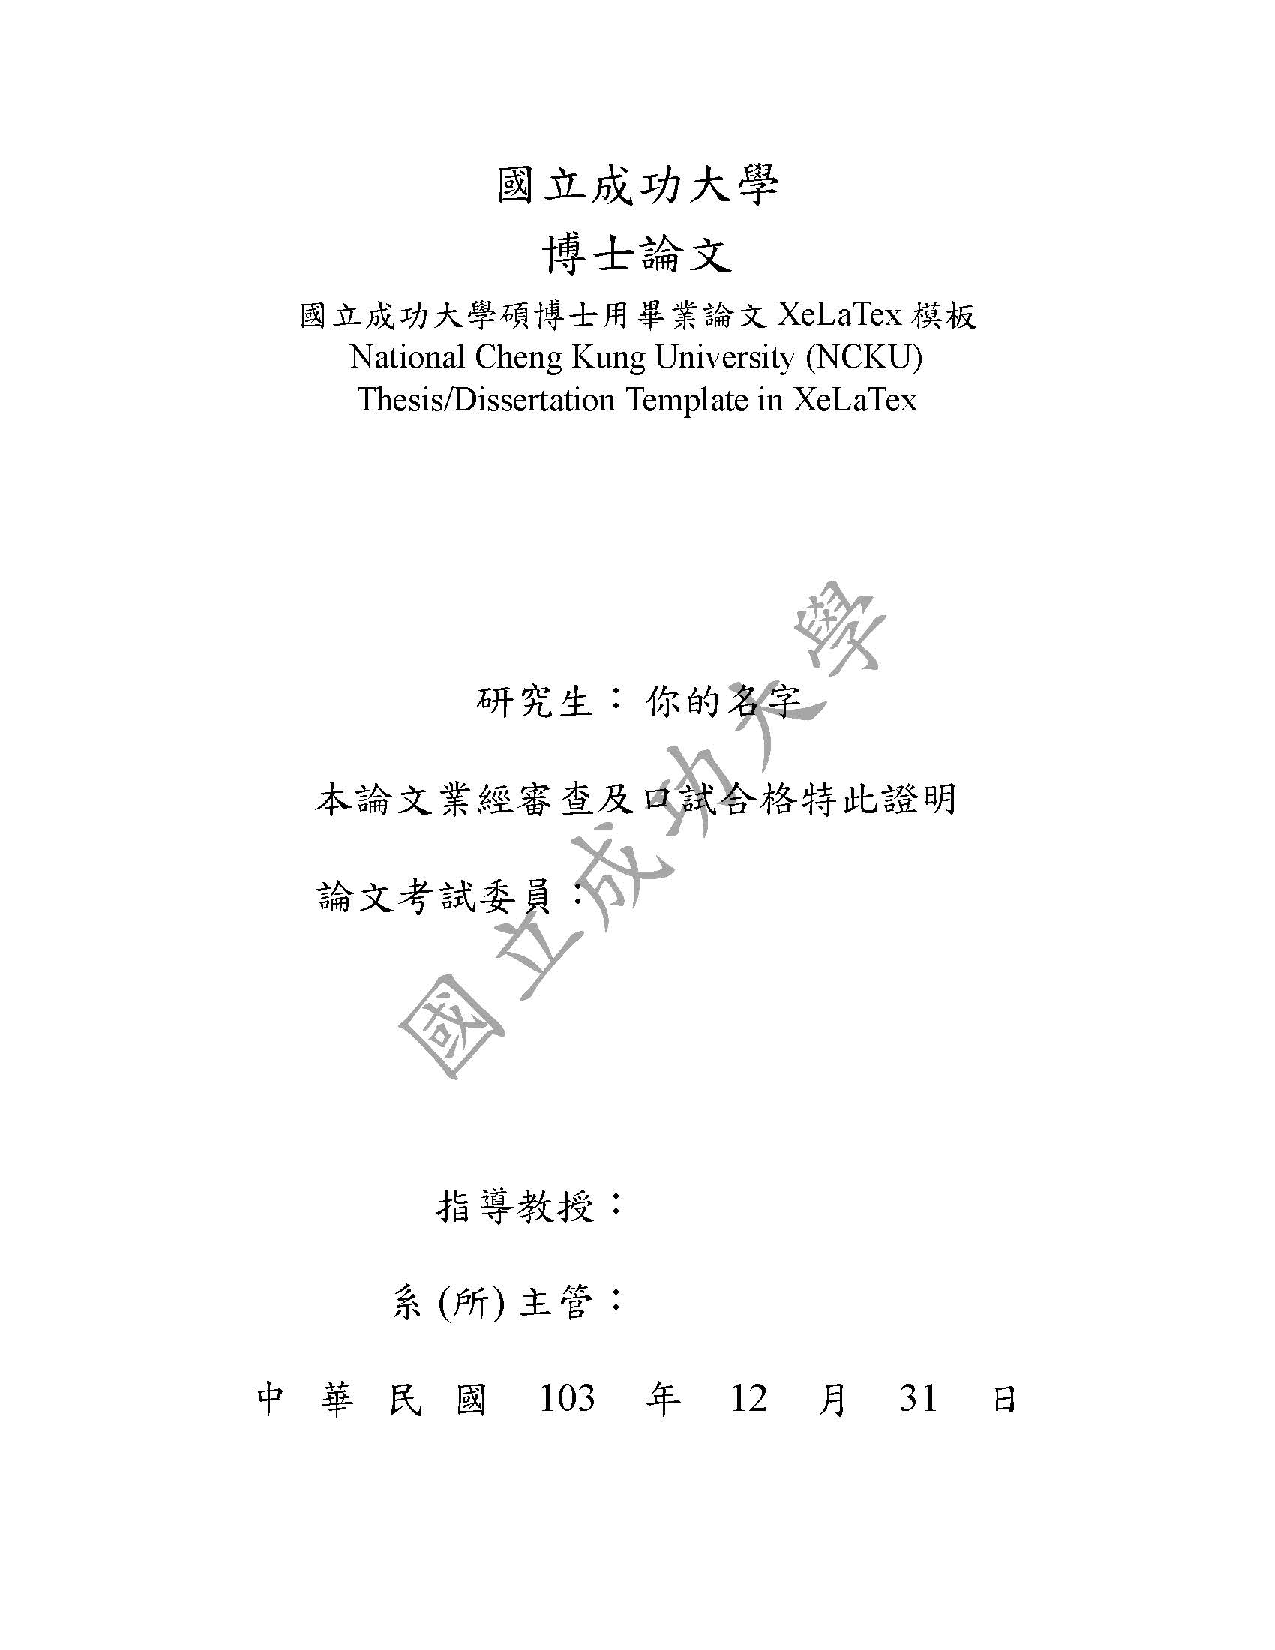
\includepdf{./oral/oral-chi.pdf}

    % ------------------------------------------------

    % English page start
    \newpage
    \phantomsection
    \addcontentsline{toc}{section}{English version}
  } % End of if{}
  {} % End of else{}

  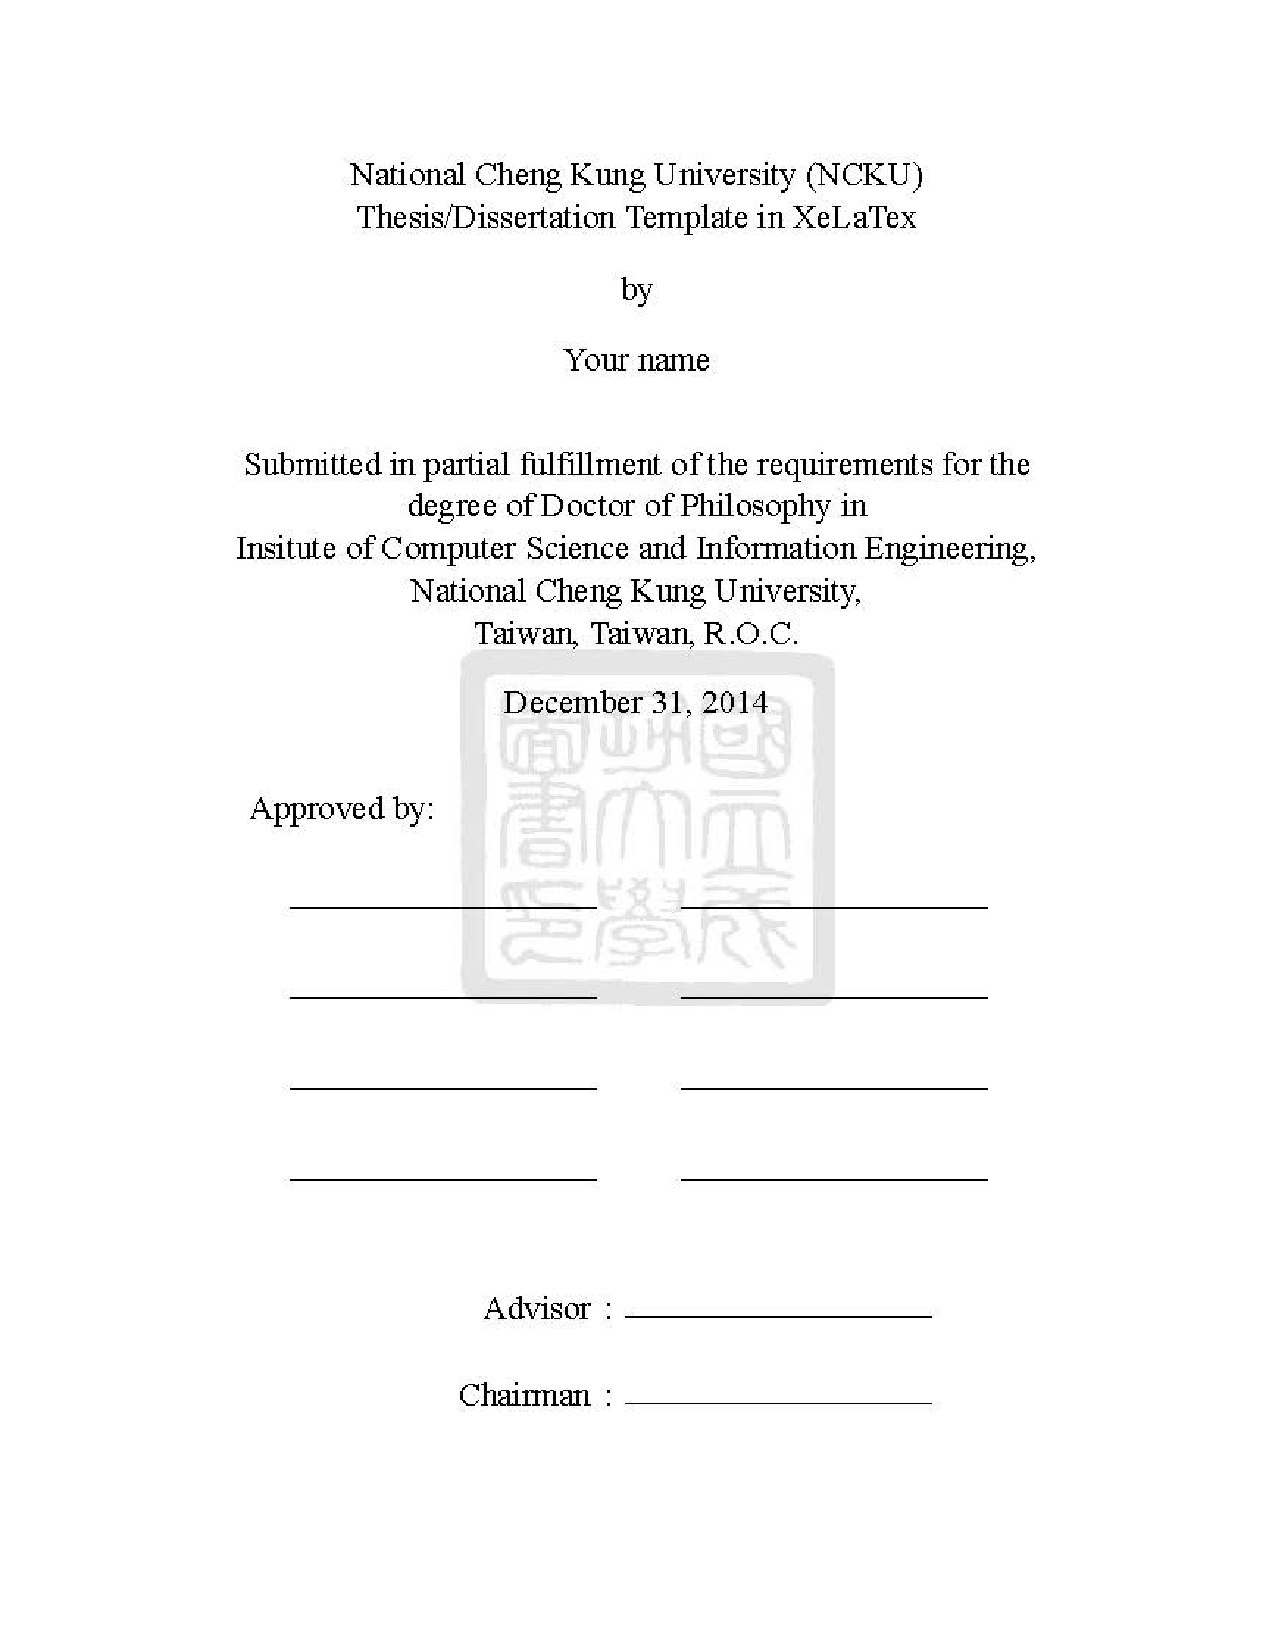
\includepdf{./oral/oral-eng.pdf}
} % End of else{}

% ----------------------------------------------------------------------------

% End of page
